
The system used in the experiment is composed by a non-anthropomorphic platform and software architecture that enrich robot's movements with emotion. The robotic platform was envisioned to be as simple as possible to limit the influence of shape on the study of the desired characteristics. 

%%%%%%%%%%%%%%%%%%%%%%%
\subsection{Hardware and Mechanical}

A holonomic platform was built to be used in the experiment. This type of platforms are characterized by the possibility to move in any direction without the necessity to have a specific orientation, i.e., they are free to move taking any desired orientation. Therefore, it was possible to imitate movements that are done by humans. For example, people do not have constaraints in movement, and can take any direction in any moment. The platform has a diameter of 25 cm and height of 25 cm. Figure~\ref{fig:ThirdDesign} shows the platform's blue prints and the real platform. Robot's frame of reference, in which all the velocities are going to be calculated, is depicted by the two black arrows. Therefore, as it could be observed, to make the robot move forward a velocity along the $y$ axis is selected by the control system.

\begin{figure}
	\centering
	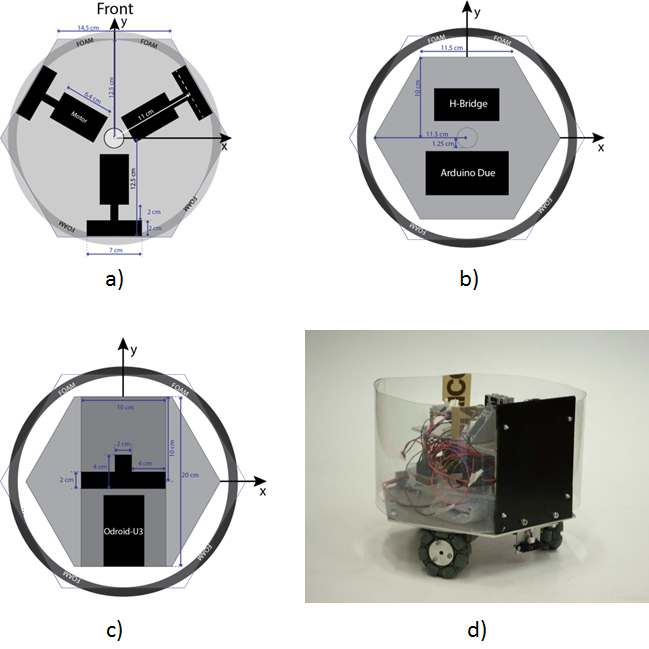
\includegraphics[width=0.48\textwidth]{Images/DesignThird.png} 
	\caption{Design of the platform. a) Base platform, this layer is used to carry the batteries. The two black arrows represent robot's frame of reference. b) First layer, which includes Arduino and the H-Bridges to control the motors. c) Second layer with Odroid-U3 and the mechanical structure to support the upper part. d) Lateral view of the robot.}
	\label{fig:ThirdDesign}
\end{figure}

%%%%%%%%%%%%%%%%%%%%%%%platform_base
\subsection{Software}
To guarantee that the correct robot's velocity for each motor could be achieved, a PID controller was implemented. PID's sets the velocity  that each motor must maintain when the platform receives a high level command. To maintain the velocity, the PID uses the velocity calculated using the odometry. Figure~\ref{fig:distribution} the general distribution of all the components, which include kinematics calculation, motors' velocity and platform velocity. 

\begin{figure}
	\centering
	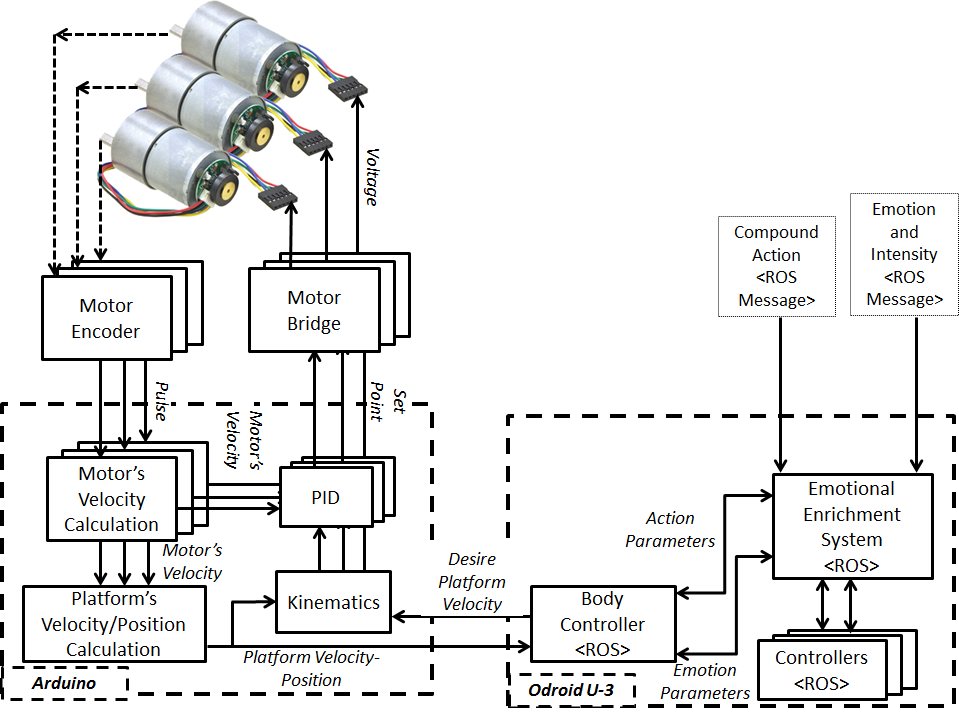
\includegraphics[width=0.45\textwidth]{Images/version-2-program.png} 
	\caption{General distribution and communication scheme among the diverse software components running on the Arduino.}
	\label{fig:distribution}
\end{figure}

Two commands could be received,  the first command specifies robot's velocities ($<V_x,V_y,\omega>$), given in robot's reference frame. The second command is a set point ($<x, Y, \theta>$) to be reached, given in the world reference frame. This world frame of reference is set every time the system is reset or boot. For example, if the robot finishes a trajectory and then it is reset, the new frame is going to be in the robot's current position.